\documentclass[12pt,a4paper,oneside]{report}             % Single-side
%\documentclass[11pt,a4paper,twoside,openright]{report}  % Duplex

% thanks to http://tex.stackexchange.com/a/47579/71109
\usepackage{ifxetex}
\usepackage{ifluatex}
\newif\ifxetexorluatex % a new conditional starts as false
\ifnum 0\ifxetex 1\fi\ifluatex 1\fi>0
   \xetexorluatextrue
\fi

\ifxetexorluatex
  \usepackage{fontspec}
\else
  \usepackage[T1]{fontenc}
  \usepackage[utf8]{inputenc}
  \usepackage[lighttt]{lmodern}
\fi

\usepackage[english,magyar]{babel} % Alapértelmezés szerint utoljára definiált nyelv lesz aktív, de később külön beállítjuk az aktív nyelvet.

\usepackage{emptypage} % omit page number on empty pages

%\usepackage{cmap}
\usepackage{amsfonts,amsmath,amssymb} % Mathematical symbols.
%\usepackage[ruled,boxed,resetcount,linesnumbered]{algorithm2e} % For pseudocodes. % beware: this is not compatible with LuaLaTeX, see http://tex.stackexchange.com/questions/34814/lualatex-and-algorithm2e
\usepackage{booktabs} % For publication quality tables for LaTeX
\usepackage{graphicx}

%\usepackage{fancyhdr}
%\usepackage{lastpage}

\usepackage{anysize}
%\usepackage{sectsty}
\usepackage{setspace} % For setting line spacing

\usepackage[unicode]{hyperref} % For hyperlinks in the generated document.
\usepackage{xcolor}
\usepackage{listings} % For source code snippets.

\usepackage[amsmath,thmmarks]{ntheorem} % Theorem-like environments.

\usepackage[hang]{caption}

\singlespacing

\newcommand{\selecthungarian}{
	\selectlanguage{magyar}
	\setlength{\parindent}{2em}
	\setlength{\parskip}{0em}
	\frenchspacing
}

\newcommand{\selectenglish}{
	\selectlanguage{english}
	\setlength{\parindent}{0em}
	\setlength{\parskip}{0.5em}
	\nonfrenchspacing
	\renewcommand{\figureautorefname}{Figure}
	\renewcommand{\tableautorefname}{Table}
	\renewcommand{\partautorefname}{Part}
	\renewcommand{\chapterautorefname}{Chapter}
	\renewcommand{\sectionautorefname}{Section}
	\renewcommand{\subsectionautorefname}{Section}
	\renewcommand{\subsubsectionautorefname}{Section}
}

\usepackage[numbers]{natbib}
\usepackage{xspace}


%TODO Set the main variables
\newcommand{\vikszerzoVezeteknev}{Ábrahám}
\newcommand{\vikszerzoKeresztnev}{Dániel}

\newcommand{\vikkonzulensAMegszolitas}{dr.~}
\newcommand{\vikkonzulensAVezeteknev}{Vörös}
\newcommand{\vikkonzulensAKeresztnev}{András}

\newcommand{\vikkonzulensBMegszolitas}{}
\newcommand{\vikkonzulensBVezeteknev}{Suszter}
\newcommand{\vikkonzulensBKeresztnev}{Máté}

\newcommand{\vikkonzulensCMegszolitas}{}
\newcommand{\vikkonzulensCVezeteknev}{}
\newcommand{\vikkonzulensCKeresztnev}{}

\newcommand{\vikcim}{Vasúti fékrendszer modellezése és megbízhatósági vizsgálata} % Cím
\newcommand{\viktanszek}{\bmemit} % Tanszék
\newcommand{\vikdoktipus}{\bsc} % Dokumentum típusa (\bsc vagy \msc)
\newcommand{\vikmunkatipusat}{szakdolgozatot} % a "hallgató nyilatkozat" részhez: szakdolgozatot vagy diplomatervet

%--------------------------------------------------------------------------------------
% TDK-specifikus változók
%--------------------------------------------------------------------------------------
\newcommand{\tdkszerzoB}{Második Szerző} % Második szerző neve; hagyd üresen, ha egyedül írtad a TDK-t.
\newcommand{\tdkev}{2014} % A dolgozat írásának éve (pl. "2014") (Ez OTDK-nál eltérhet az aktuális évtől.)

% További adatok az OTDK címlaphoz (BME-s TDK-hoz nem kell kitölteni)
\newcommand{\tdkevfolyamA}{IV} % Első szerző évfolyama, római számmal (pl. IV).
\newcommand{\tdkevfolyamB}{III} % Második szerző évfolyama, római számmal (pl. III).
\newcommand{\tdkkonzulensbeosztasA}{egyetemi tanár} % Első konzulens beosztása (pl. egyetemi docens)
\newcommand{\tdkkonzulensbeosztasB}{doktorandusz} % Második konzulens beosztása (pl. egyetemi docens)

\newcommand{\szerzoMeta}{\vikszerzoVezeteknev{} \vikszerzoKeresztnev} % egy szerző esetén
%\newcommand{\szerzoMeta}{\vikszerzoVezeteknev{} \vikszerzoKeresztnev, \tdkszerzoB} % két szerző esetén

%TODO Language configuration -- choose one
% Beállítások magyar nyelvű dolgozathoz
%--------------------------------------------------------------------------------------
% Elnevezések
%--------------------------------------------------------------------------------------
\newcommand{\bme}{Budapesti Műszaki és Gazdaságtudományi Egyetem}
\newcommand{\vik}{Villamosmérnöki és Informatikai Kar}

\newcommand{\bmemit}{Méréstechnika és Információs Rendszerek Tanszék}

\newcommand{\keszitette}{Készítette}
\newcommand{\konzulens}{Konzulens}

\newcommand{\bsc}{Szakdolgozat}
\newcommand{\msc}{Diplomaterv}
\newcommand{\tdk}{TDK dolgozat}
\newcommand{\bsconlab}{BSc Önálló laboratórium}
\newcommand{\msconlabi}{MSc Önálló laboratórium 1.}
\newcommand{\msconlabii}{MSc Önálló laboratórium 2.}

\newcommand{\pelda}{Példa}
\newcommand{\definicio}{Definíció}
\newcommand{\tetel}{Tétel}

\newcommand{\bevezetes}{Bevezetés}
\newcommand{\koszonetnyilvanitas}{Köszönetnyilvánítás}
\newcommand{\fuggelek}{Függelék}

% Opcionálisan átnevezhető címek
%\addto\captionsmagyar{%
%\renewcommand{\listfigurename}{Saját ábrajegyzék cím}
%\renewcommand{\listtablename}{Saját táblázatjegyzék cím}
%\renewcommand{\bibname}{Saját irodalomjegyzék név}
%}

\newcommand{\szerzo}{\vikszerzoVezeteknev{} \vikszerzoKeresztnev}
\newcommand{\vikkonzulensA}{\vikkonzulensAMegszolitas\vikkonzulensAVezeteknev{} \vikkonzulensAKeresztnev}
\newcommand{\vikkonzulensB}{\vikkonzulensBMegszolitas\vikkonzulensBVezeteknev{} \vikkonzulensBKeresztnev}
\newcommand{\vikkonzulensC}{\vikkonzulensCMegszolitas\vikkonzulensCVezeteknev{} \vikkonzulensCKeresztnev}

\newcommand{\selectthesislanguage}{\selecthungarian}

\bibliographystyle{huplain}

\def\lstlistingname{lista}

\newcommand{\appendixnumber}{6}  % a fofejezet-szamlalo az angol ABC 6. betuje (F) lesz

% Settings for English documents
%%--------------------------------------------------------------------------------------
% Elnevezések
%--------------------------------------------------------------------------------------
\newcommand{\bme}{Budapest University of Technology and Economics}
\newcommand{\vik}{Faculty of Electrical Engineering and Informatics}

\newcommand{\bmemit}{Department of Measurement and Information Systems}

\newcommand{\keszitette}{Author}
\newcommand{\konzulens}{Advisor}

\newcommand{\bsc}{Bachelor's Thesis}
\newcommand{\msc}{Master's Thesis}
\newcommand{\tdk}{Scientific Students' Association Report}
\newcommand{\bsconlab}{BSc Project Laboratory}
\newcommand{\msconlabi}{MSc Project Laboratory 1}
\newcommand{\msconlabii}{MSc Project Laboratory 2}

\newcommand{\pelda}{Example}
\newcommand{\definicio}{Definition}
\newcommand{\tetel}{Theorem}

\newcommand{\bevezetes}{Introduction}
\newcommand{\koszonetnyilvanitas}{Acknowledgements}
\newcommand{\fuggelek}{Appendix}

% Optional custom titles
%\addto\captionsenglish{%
%\renewcommand*{\listfigurename}{Your list of figures title}
%\renewcommand*{\listtablename}{Your list of tables title}
%\renewcommand*{\bibname}{Your bibliography title}
%}

\newcommand{\szerzo}{\vikszerzoKeresztnev{} \vikszerzoVezeteknev}
\newcommand{\vikkonzulensA}{\vikkonzulensAMegszolitas\vikkonzulensAKeresztnev{} \vikkonzulensAVezeteknev}
\newcommand{\vikkonzulensB}{\vikkonzulensBMegszolitas\vikkonzulensBKeresztnev{} \vikkonzulensBVezeteknev}
\newcommand{\vikkonzulensC}{\vikkonzulensCMegszolitas\vikkonzulensCKeresztnev{} \vikkonzulensCVezeteknev}

\newcommand{\selectthesislanguage}{\selectenglish}

\bibliographystyle{plainnat}

\newcommand{\ie}{i.e.\@\xspace}
\newcommand{\Ie}{I.e.\@\xspace}
\newcommand{\eg}{e.g.\@\xspace}
\newcommand{\Eg}{E.g.\@\xspace}
\newcommand{\etal}{et al.\@\xspace}
\newcommand{\etc}{etc.\@\xspace}
\newcommand{\vs}{vs.\@\xspace}
\newcommand{\viz}{viz.\@\xspace} % videlicet
\newcommand{\cf}{cf.\@\xspace} % confer
\newcommand{\Cf}{Cf.\@\xspace}
\newcommand{\wrt}{w.r.t.\@\xspace} % with respect to
\newcommand{\approximately}{approx.\xspace}

\newcommand{\appendixnumber}{1}  % a fofejezet-szamlalo az angol ABC 1. betuje (A) lesz


%--------------------------------------------------------------------------------------
% Page layout setup
%--------------------------------------------------------------------------------------
% we need to redefine the pagestyle plain
% another possibility is to use the body of this command without \fancypagestyle
% and use \pagestyle{fancy} but in that case the special pages
% (like the ToC, the References, and the Chapter pages)remain in plane style

\pagestyle{plain}
\marginsize{35mm}{25mm}{15mm}{15mm}

\setcounter{tocdepth}{3}
%\sectionfont{\large\upshape\bfseries}
\setcounter{secnumdepth}{3}

\sloppy % Margón túllógó sorok tiltása.
\widowpenalty=10000 \clubpenalty=10000 %A fattyú- és árvasorok elkerülése
\def\hyph{-\penalty0\hskip0pt\relax} % Kötőjeles szavak elválasztásának engedélyezése


%--------------------------------------------------------------------------------------
% Setup hyperref package
%--------------------------------------------------------------------------------------
\hypersetup{
    % bookmarks=true,            % show bookmarks bar?
    unicode=true,              % non-Latin characters in Acrobat's bookmarks
    pdftitle={\vikcim},        % title
    pdfauthor={\szerzoMeta},    % author
    pdfsubject={\vikdoktipus}, % subject of the document
    pdfcreator={\szerzoMeta},   % creator of the document
    pdfproducer={},    % producer of the document
    pdfkeywords={},    % list of keywords (separate then by comma)
    pdfnewwindow=true,         % links in new window
    colorlinks=true,           % false: boxed links; true: colored links
    linkcolor=black,           % color of internal links
    citecolor=black,           % color of links to bibliography
    filecolor=black,           % color of file links
    urlcolor=black             % color of external links
}


%--------------------------------------------------------------------------------------
% Set up listings
%--------------------------------------------------------------------------------------
\definecolor{lightgray}{rgb}{0.95,0.95,0.95}
\lstset{
	basicstyle=\scriptsize\ttfamily, % print whole listing small
	keywordstyle=\color{black}\bfseries, % bold black keywords
	identifierstyle=, % nothing happens
	% default behavior: comments in italic, to change use
	% commentstyle=\color{green}, % for e.g. green comments
	stringstyle=\scriptsize,
	showstringspaces=false, % no special string spaces
	aboveskip=3pt,
	belowskip=3pt,
	backgroundcolor=\color{lightgray},
	columns=flexible,
	keepspaces=true,
	escapeinside={(*@}{@*)},
	captionpos=b,
	breaklines=true,
	frame=single,
	float=!ht,
	tabsize=2,
	literate=*
		{á}{{\'a}}1	{é}{{\'e}}1	{í}{{\'i}}1	{ó}{{\'o}}1	{ö}{{\"o}}1	{ő}{{\H{o}}}1	{ú}{{\'u}}1	{ü}{{\"u}}1	{ű}{{\H{u}}}1
		{Á}{{\'A}}1	{É}{{\'E}}1	{Í}{{\'I}}1	{Ó}{{\'O}}1	{Ö}{{\"O}}1	{Ő}{{\H{O}}}1	{Ú}{{\'U}}1	{Ü}{{\"U}}1	{Ű}{{\H{U}}}1
}


%--------------------------------------------------------------------------------------
% Set up theorem-like environments
%--------------------------------------------------------------------------------------
% Using ntheorem package -- see http://www.math.washington.edu/tex-archive/macros/latex/contrib/ntheorem/ntheorem.pdf

\theoremstyle{plain}
\theoremseparator{.}
\newtheorem{example}{\pelda}

\theoremseparator{.}
%\theoremprework{\bigskip\hrule\medskip}
%\theorempostwork{\hrule\bigskip}
\theorembodyfont{\upshape}
\theoremsymbol{{\large \ensuremath{\centerdot}}}
\newtheorem{definition}{\definicio}

\theoremseparator{.}
%\theoremprework{\bigskip\hrule\medskip}
%\theorempostwork{\hrule\bigskip}
\newtheorem{theorem}{\tetel}


%--------------------------------------------------------------------------------------
% Some new commands and declarations
%--------------------------------------------------------------------------------------
\newcommand{\code}[1]{{\upshape\ttfamily\scriptsize\indent #1}}
\newcommand{\doi}[1]{DOI: \href{http://dx.doi.org/\detokenize{#1}}{\raggedright{\texttt{\detokenize{#1}}}}} % A hivatkozások közt így könnyebb DOI-t megadni.

\DeclareMathOperator*{\argmax}{arg\,max}
%\DeclareMathOperator*[1]{\floor}{arg\,max}
\DeclareMathOperator{\sign}{sgn}
\DeclareMathOperator{\rot}{rot}


%--------------------------------------------------------------------------------------
% Setup captions
%--------------------------------------------------------------------------------------
\captionsetup[figure]{aboveskip=10pt}

\renewcommand{\captionlabelfont}{\bf}
%\renewcommand{\captionfont}{\footnotesize\it}

%--------------------------------------------------------------------------------------
% Hyphenation exceptions
%--------------------------------------------------------------------------------------
\hyphenation{Shakes-peare Mar-seilles ár-víz-tű-rő tü-kör-fú-ró-gép}


\author{\vikszerzo}
\title{\viktitle}


%--------------------------------------------------------------------------------------
% Table of contents and the main text
%--------------------------------------------------------------------------------------
\begin{document}

\pagenumbering{gobble}

%TODO These includes define guidelines -- remove these
%~~~~~~~~~~~~~~~~~~~~~~~~~~~~~~~~~~~~~~~~~~~~~~~~~~~~~~~~~~~~~~~~~~~~~~~~~~~~~~~~~~~~~~
%\selecthungarian
%--------------------------------------------------------------------------------------
% Rovid formai es tartalmi tajekoztato
%--------------------------------------------------------------------------------------

\footnotesize
\begin{center}
\large
\textbf{\Large Általános információk, a diplomaterv szerkezete}\\
\end{center}

A diplomaterv szerkezete a BME Villamosmérnöki és Informatikai Karán:
\begin{enumerate}
\item	Diplomaterv feladatkiírás
\item	Címoldal
\item	Tartalomjegyzék
\item	A diplomatervező nyilatkozata az önálló munkáról és az elektronikus adatok kezeléséről
\item	Tartalmi összefoglaló magyarul és angolul
\item	Bevezetés: a feladat értelmezése, a tervezés célja, a feladat indokoltsága, a diplomaterv felépítésének rövid összefoglalása
\item	A feladatkiírás pontosítása és részletes elemzése
\item	Előzmények (irodalomkutatás, hasonló alkotások), az ezekből levonható következtetések
\item	A tervezés részletes leírása, a döntési lehetőségek értékelése és a választott megoldások indoklása
\item	A megtervezett műszaki alkotás értékelése, kritikai elemzése, továbbfejlesztési lehetőségek
\item	Esetleges köszönetnyilvánítások
\item	Részletes és pontos irodalomjegyzék
\item	Függelék(ek)
\end{enumerate}

Felhasználható a következő oldaltól kezdődő \LaTeX diplomatervsablon dokumentum tartalma. 

A diplomaterv szabványos méretű A4-es lapokra kerüljön. Az oldalak tükörmargóval készüljenek (mindenhol 2,5~cm, baloldalon 1~cm-es kötéssel). Az alapértelmezett betűkészlet a 12 pontos Times New Roman, másfeles sorközzel, de ettől kismértékben el lehet térni, ill. más betűtípus használata is megengedett.

Minden oldalon -- az első négy szerkezeti elem kivételével -- szerepelnie kell az oldalszámnak.

A fejezeteket decimális beosztással kell ellátni. Az ábrákat a megfelelő helyre be kell illeszteni, fejezetenként decimális számmal és kifejező címmel kell ellátni. A fejezeteket decimális aláosztással számozzuk, maximálisan 3 aláosztás mélységben (pl. 2.3.4.1.). Az ábrákat, táblázatokat és képleteket célszerű fejezetenként külön számozni (pl. 2.4. ábra, 4.2. táblázat vagy képletnél (3.2)). A fejezetcímeket igazítsuk balra, a normál szövegnél viszont használjunk sorkiegyenlítést. Az ábrákat, táblázatokat és a hozzájuk tartozó címet igazítsuk középre. A cím a jelölt rész alatt helyezkedjen el.

A képeket lehetőleg rajzoló programmal készítsék el, az egyenleteket egyenlet-szerkesztő segítségével írják le (A \LaTeX~ehhez kézenfekvő megoldásokat nyújt).

Az irodalomjegyzék szövegközi hivatkozása történhet sorszámozva (ez a preferált megoldás) vagy a Harvard-rendszerben (a szerző és az évszám megadásával). A teljes lista névsor szerinti sorrendben a szöveg végén szerepeljen (sorszámozott irodalmi hivatkozások esetén hivatkozási sorrendben). A szakirodalmi források címeit azonban mindig az eredeti nyelven kell megadni, esetleg zárójelben a fordítással. A listában szereplő valamennyi publikációra hivatkozni kell a szövegben (a \LaTeX-sablon a Bib\TeX~segítségével mindezt automatikusan kezeli). Minden publikáció a szerzők után a következő adatok szerepelnek: folyóirat cikkeknél a pontos cím, a folyóirat címe, évfolyam, szám, oldalszám tól-ig. A folyóiratok címét csak akkor rövidítsük, ha azok nagyon közismertek vagy nagyon hosszúak. Internetes hivatkozások megadásakor fontos, hogy az elérési út előtt megadjuk az oldal tulajdonosát és tartalmát (mivel a link egy idő után akár elérhetetlenné is válhat), valamint az elérés időpontját.

\vspace{5mm}
Fontos:
\begin{itemize}
	\item A szakdolgozatkészítő / diplomatervező nyilatkozata (a jelen sablonban szereplő szövegtartalommal) kötelező előírás, Karunkon ennek hiányában a szakdolgozat/diplomaterv nem bírálható és nem védhető!
	\item Mind a dolgozat, mind a melléklet maximálisan 15~MB méretű lehet!
\end{itemize}

\vspace{5mm}
\begin{center}
Jó munkát, sikeres szakdolgozatkészítést, ill. diplomatervezést kívánunk!
\end{center}

\normalsize
\selectthesislanguage

%%--------------------------------------------------------------------------------------
% Feladatkiiras (a tanszeken atveheto, kinyomtatott valtozat)
%--------------------------------------------------------------------------------------
\clearpage
\begin{center}
\large
\textbf{FELADATKIÍRÁS}\\
\end{center}

A feladatkiírást a tanszéki adminisztrációban lehet átvenni, és a leadott munkába eredeti, tanszéki pecséttel ellátott és a tanszékvezető által aláírt lapot kell belefűzni (ezen oldal \emph{helyett}, ez az oldal csak útmutatás). Az elektronikusan feltöltött dolgozatban már nem kell beleszerkeszteni ezt a feladatkiírást.


\selectthesislanguage

%TODO Titlepage -- choose one from below
%~~~~~~~~~~~~~~~~~~~~~~~~~~~~~~~~~~~~~~~~~~~~~~~~~~~~~~~~~~~~~~~~~~~~~~~~~~~~~~~~~~~~~~
\include{include/titlepage}		   % Szakdolgozat/Diplomaterv címlap
%%% TDK címlap
\begin{titlepage}
  \begin{center}  
  \includegraphics[width=7cm]{./figures/bme_logo.pdf}
  \vspace{0.3cm}
  
  \bme \\
  \vik \\
  \viktanszek \\
  \vspace{5cm}
  
  \huge {\vikcim}
  \vspace{1.5cm}
  
  \large {\textbf{\tdk}}
  \vfill
    
  {\Large 
  	\keszitette: \\ \vspace{0.3cm}
  	\szerzo \\
	\tdkszerzoB \\
  	\vspace{1.5cm}
  	\konzulens: \\ \vspace{0.3cm}
  	\vikkonzulensA \\
  	\vikkonzulensB \\
  }
  
  \vspace{2cm}
  \large {\tdkev}
 \end{center}
\end{titlepage}
%% Címlap vége
	% TDK címlap
%\include{include/titlepage-otdk}   % OTDK címlap


% Table of Contents
%~~~~~~~~~~~~~~~~~~~~~~~~~~~~~~~~~~~~~~~~~~~~~~~~~~~~~~~~~~~~~~~~~~~~~~~~~~~~~~~~~~~~~~
\tableofcontents\cleardoublepage


% Declaration and Abstract
%~~~~~~~~~~~~~~~~~~~~~~~~~~~~~~~~~~~~~~~~~~~~~~~~~~~~~~~~~~~~~~~~~~~~~~~~~~~~~~~~~~~~~~
\selectlanguage{magyar}
\pagenumbering{gobble}
%--------------------------------------------------------------------------------------
% Nyilatkozat
%--------------------------------------------------------------------------------------
\begin{center}
\large
\textbf{HALLGATÓI NYILATKOZAT}\\
\end{center}

Alulírott \emph{\vikszerzoVezeteknev{} \vikszerzoKeresztnev}, szigorló hallgató kijelentem, hogy ezt a \vikmunkatipusat{} meg nem engedett segítség nélkül, saját magam készítettem, csak a megadott forrásokat (szakirodalom, eszközök stb.) használtam fel. Minden olyan részt, melyet szó szerint, vagy azonos értelemben, de átfogalmazva más forrásból átvettem, egyértelműen, a forrás megadásával megjelöltem.

Hozzájárulok, hogy a jelen munkám alapadatait (szerző(k), cím, angol és magyar nyelvű tartalmi kivonat, készítés éve, konzulens(ek) neve) a BME VIK nyilvánosan hozzáférhető elektronikus formában, a munka teljes szövegét pedig az egyetem belső hálózatán keresztül (vagy autentikált felhasználók számára) közzétegye. Kijelentem, hogy a benyújtott munka és annak elektronikus verziója megegyezik. Dékáni engedéllyel titkosított diplomatervek esetén a dolgozat szövege csak 3 év eltelte után válik hozzáférhetővé.

\begin{flushleft}
\vspace*{1cm}
Budapest, \today
\end{flushleft}

\begin{flushright}
 \vspace*{1cm}
 \makebox[7cm]{\rule{6cm}{.4pt}}\\
 \makebox[7cm]{\emph{\vikszerzoVezeteknev{} \vikszerzoKeresztnev}}\\
 \makebox[7cm]{hallgató}
\end{flushright}
\thispagestyle{empty}

\vfill
\cleardoublepage

\selectthesislanguage
 %TODO Hallgatói nyilatkozat -- TDK és OTDK esetén törlendő!
\pagenumbering{roman}
\setcounter{page}{1}

\selecthungarian

%----------------------------------------------------------------------------
% Abstract in Hungarian
%----------------------------------------------------------------------------
\chapter*{Kivonat}\addcontentsline{toc}{chapter}{Kivonat}



\vfill
%\selectenglish


%----------------------------------------------------------------------------
% Abstract in English
%----------------------------------------------------------------------------
%\chapter*{Abstract}\addcontentsline{toc}{chapter}{Abstract}

%This document is a \LaTeX-based skeleton for BSc/MSc~theses of students at the Electrical Engineering and Informatics Faculty, Budapest University of Technology and Economics. The usage of this skeleton is optional. It has been tested with the \emph{TeXLive} \TeX~implementation, and it requires the PDF-\LaTeX~compiler.


%\vfill
\cleardoublepage

\selectthesislanguage

\newcounter{romanPage}
\setcounter{romanPage}{\value{page}}
\stepcounter{romanPage}    %TODO Összefoglaló -- TDK és OTDK esetén nem kötelező


% The main part of the thesis
%~~~~~~~~~~~~~~~~~~~~~~~~~~~~~~~~~~~~~~~~~~~~~~~~~~~~~~~~~~~~~~~~~~~~~~~~~~~~~~~~~~~~~~
\pagenumbering{arabic}

%TODO import your own content
%----------------------------------------------------------------------------
\chapter{\bevezetes}
%----------------------------------------------------------------------------

A bevezető tartalmazza a diplomaterv-kiírás elemzését, történelmi előzményeit, a feladat indokoltságát (a motiváció leírását), az eddigi megoldásokat, és ennek tükrében a hallgató megoldásának összefoglalását.

A bevezető szokás szerint a diplomaterv felépítésével záródik, azaz annak rövid leírásával, hogy melyik fejezet mivel foglalkozik. \cite{Mkrtychev:1997}

%-----------------------------------------------------------
\chapter{\hatterismeret}\label{chap:hatter}
%-----------------------------------------------------------

\section{Modellezés}
\subsection{Modell-alapú rendszerfejlesztés}
A modell-alapú rendszerfejsztés, angolul rövidítve MBSE\footnote{Model-based systems engineering}, egy formalizált módszertan, amely a követelméynkezelés, tervezés, analízis, verifikáció és validáció témaköreiben nyújt segítséget az összetett rendszerek fejlesztése során.
A dokumentum-alapú fejlesztéssel ellentétben az MBSE modelleket helyez a fejlesztés középpontjába.
A 2020-as évben a NASA\footnote{National Aeronautics and Space Administration, Amerikai Egyesült Államok kormányzati ügynöksége} is megjegyezte, hogy ,,A modell-alapú rendszertervezést mind az ipari mind a kormányzati egyre inkább felkarolja, hogy lépést tudjon tartani a rendszer komplexitásával.''\cite{Nasa2020}
Az MBSE három különböző koncepciót hoz össze: modell, rendszergondolkodás, rendszerfejlesztés (Shevchenko, 2020 \cite{shevchenko_2020})

A modell-alapú rendszerfejlesztés növelheti az a teljes termék specifikációhoz tartozó információ megragadásának, vizsgálatának, megosztásának és koordinálásának képességét, amely a következő előnyökkel járhat (Friedenthal, 2007 \cite{friedenthal2007incose}):
\begin{itemize}
    \item Javítja a kommunikációt a fejlesztésben részvevők között (például: a vevő, a projekt vezető, a rendszermérnökök, hardver és szoftver fejlesztők, tesztelők stb.).
    \item Az összetettség menedzselésének javítása.
    \item Megnövekedett termék minőség.
    \item A rendszertervezés alapjainak tanítási és tanulási képességének javulása.
\end{itemize}

Manapság a modell-alapú rendszertervezés számos iparágban jelen van, például: Járműipar, közlekedés, űripar, orvosi eszközök, robotika, nukleáris technológia, ipari rendszrek, gyártás stb.
Leginkább olyan környezetekben használatos, ahol valóság korlátos (beavatkozás behatárolt, méret kényszer stb.), 
fontos az együttműködés több szakmán/beszállítókon keresztül, 
drága a prototípus gyártás vagy biztonságkritikus rendszereknél (Molnár, 2019 \cite{rete0}).

\subsection{SysML}
A SysML\footnote{Systems Modeling Language} egy általános célú architektúra modellező nyelv rendszermérnöki felhasználásra.
A nyelv támogja számos rendszerek, rendszerek rendszereinek (Systems of systems) specifikálását, vizsgálatát, tervezését, verifikációját és validációját.
Ezek tartalmazhatnak hardver/szoftver elemeket, információkat, folyamatokat, személyzetet és létesítményeket.
A SysML az UML\footnote{Unified Modeling Language} 2-nek egy dialektusa és egy UML 2 Profilként van definiálva \cite{sysml}.

A SysML Cris Kobryn által szervezett rendszermérnökökből és modellező eszköz szakértőkből álló informális szövettség úgy nevezett ,,SysML Partnekek'' által lett létrehozva 2003-ban.
Az első kiadás 2005-ben jelent meg és az elsődleges közreműködök között ott volt a Motorola, a Telelogic és a Northrop Grumman is.
Másfél évvel az első megjelenés után, 2006-ban hivatalosan is adaptálásra került a specifikáció az OMG\footnote{Object Management Group} által, ezáltal a specifikáció hivatalos neve: OMG SysML 1.0.
A mai napig nem történt nagy változás a szabványban. A jelenleg használt legfrissebb verzió az 1.5-ös, bár az OMG 2017-ben benyújtott egy változtatást OMG SysML 2.0 néven \cite{sysml-partner}.

\subsubsection{Modell elemek}
Mint az már fentebb említve lett, a SysML kiegészíti az UML 2 nyelvet.
A két nyelv kapcsolatát az \ref{fig:sysUML}. ábra szemlélteti.
Látható, hogy egyes elemek teljesen kikerültek a SysML eszközkészletéből, de számos újdonság került bele.

\begin{figure}
    \footnotesize
    \centering
    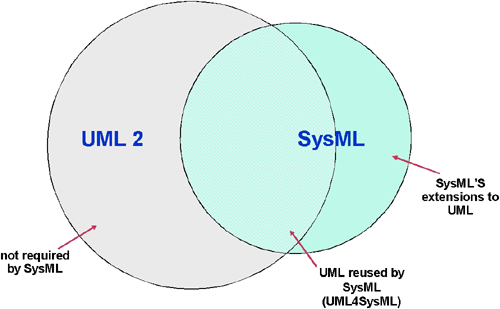
\includegraphics[width=100mm, keepaspectratio]{figures/sysml_uml.jpg}
    \caption{A SysML és az UML kapcsolata (Forrás: \cite{omgsysml})}
    \label{fig:sysUML}
\end{figure}

A SysML struktúrájának alapvető egysége a blokk, amit bármilyen rendszer elem reprezentálására lehet használni (például: hardver, szoftver, létesítmény, személyzet stb.).
A rendszerstruktúrát blokk definíciós diagrammok (BDD\footnote{Block Definition Diagram}) és ,,internal block'' diagrammok (IBD\footnote{internal block diagram}) alkotják.
A BDD írja le a rendszer hierarhiáját, míg az IDB a belső struktúrát.

A nyelv támogat számos viselkedésleíró diagrammot is. Ezek nagyrésze egyezik az UML-ben definiált párjával.
Az egyetlen kivétel az Aktivitás diagramm, amely kissé módosult az adaptáció során.

A hasonlóságokat és különbségeket legjobban az \ref{fig:sysDiag}. ábra mutatja be.

\begin{figure}
    \footnotesize
    \centering
    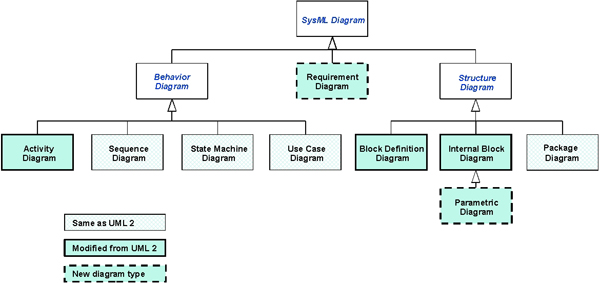
\includegraphics[width=100mm, keepaspectratio]{figures/sysml_diagrams.jpg}
    \caption{SysML diagramm típusok (Forrás: \cite{omgsysml})}
    \label{fig:sysDiag}
\end{figure}

\section{Safety modellezés}
\chapter{Irodalmi kutatás}\label{chap:irodalom}
\section{FIT Allokáció} \label{sec:fit_allocation}
Az ipari rendszerek egyre összetettebbekké váltak az évek során. 
Emellett mostanság egyre több ilyen rendszer tartalmaz elektronikát és szoftvert, 
tehát a funkcionális biztonságnak folyamatosan nő a fontossága.\cite{Schabe}

A RAMS\footnote{Reliability, Availability, Maintainability and Safety} követelmények allokációja szerves részét képezi az alacsonyabb szinten lévő alrendszerek tervezésének rendszer mérnöki folyamatoban.
A allokáció célja, hogy megtalálja a leghatékonyabb fizikai architektúrát, ami megfelel a rendszerszintű követelményeknek és az allokáció funkcionális viselkedés analizálása által szervezett.
Amikor RAMS konstukció szükséges minden teljesítménybeli követelményfajtára - megbízhatóság, elérhetőség, karbantarthatóság, biztonságosság - külön kell az allokációs folyamatot végezni.
Az allokációs módszerek a négy különböző karakterisztikára hasonlók. \cite{en60300-3-1}

Amikor az allokáció a tervezés olyan korai fázisában kezdődik, amikor még nincs elegendő rendelkezésre álló információ az allokációt folyamatosan frissíteni kell a funkcionális analízis során.
A rendszer alacsonyabb szintjein lévő allokáció szükséges a termék meghatározási fázishoz és céljaihoz \cite{en60300-1}:
\begin{itemize}
	\item Hogy igazolja a teljes rendszer RAMS követelméyneinek megvalósíthatóságát,
	\item Hogy meghatározzon ellenőrizhető RAMS design követelményeket alacsony szinten és
	\item Hogy meghatározzon egyértelmű és megvalósítható RAMS követelményeket az alrendszerek és komponensek számára.
\end{itemize}
Általánosságban az allokációs folyamat a következő lépésekből áll:
\begin{itemize}
	\item A rendszer tanulmányozása
	\item Azon területek megtalálása, ahol a terv és a hozzá tartozó RAMS karakterisztika információk elérhetők.
	\item Alkalmas súlyok hozzárendelése és
	\item Meghatározni a magasszintű követelményhez való hozzájárulását
\end{itemize}


A safety integrity level (SIL) egy diszkrét érték ami meghatározza a használandó módszereket, technikákat a véletlenszerű és szisztematikus hibák elkerülése érdekében.
A SIL-ek koncepciója már több szabvány rendszerben ki lett fejlesztve.
Ezek között legismertebb szabványok az IEC 61508, DEF-STAN-0056, EN 50126, EN 50128, EN 50129 és még sok más.

A SIL-nek két fő aspektusa van:
\begin{enumerate}
    \item Egy cél hibaráta, amit a rendszernek nem szabad meghaladni, hogy tudja kezelni a véletlen hibákat
    \item Módszerek és technikák halmaza, amit a szisztematikus hibákat kezeli 
\end{enumerate}

Itt fontos megjegyezni, hogy szoftverben csak és kizárólag szisztematikus hibákat vesznek figyelembe és nincs megadva cél hibaráta. Ez abból adódik, hogy a szoftverben nincs véletlenszerű hiba.

\subsection{Különböző SIL-ek}
A \ref{tab:SILs} táblázat példát ad a SIL-ek és a tűrhető hibaráta kapcsolatára, ahogy három szabvány, az IEC 61508, az EN 50129 és a DEF-STAN-0056 definiálja.

A tűrhető hibaráta (THR) egy eszköz veszélyes hibáinak maximális rátája, amit a szabvány definiál bizonyos safety integrity szinthez.
Látni kell azt, hogy bár az IEC és EN szabványoknál azonosak a THR értékek, a DEF-STAN-0056-ban eltér.
Ezért a szabványok közti átjárás nem mindig triviális.
Attól még, hogy a THR értékek hasonlóak az IEC és EN szabványok között, az rendszer szintű hibaelkerülő módszerek különböznek, ezért ezek a SIL-ek sem ugyan azok.
\begin{table}[ht]
	\footnotesize
	\centering
	\begin{tabular}{ l c c }
		\toprule
		SIL & IEC 61508/EN 50129 & DEF-STAN-0056 \\
		\midrule
		1 & \(10^{-6}/h \leq\) THR \(< 10^{-5}/h\) & Frequent \(\approx 10^{-2}/h\)\\
		2 & \(10^{-7}/h \leq\) THR \(< 10^{-6}/h\)  & Probable \(\approx 10^{-4}/h\)\\
		3 & \(10^{-8}/h \leq\) THR \(< 10^{-7}/h\)  & Occasional \(\approx 10^{-6}/h\)\\
		4 & \(10^{-9}/h \leq\) THR \(< 10^{-8}/h\)  & Remote \(\approx 10^{-8}/h\) \\
		\bottomrule
	\end{tabular}
	\caption{SIL értékek több szabvány és THR szerint}
	\label{tab:SILs}
\end{table}

\section{Allokációs módszerek}
MIL-HDBK-388B\cite{388B} nyújt négy módszert az allokációhoz, melyek lentebb láthatók:
\begin{itemize}
	\item Egyenlő elosztás módszer\footnote{Equal allocation technique}
	\item ARINC\footnote{Aeronautical Radio, Inc} elosztás módszer
	\item ,,Feasibility of objective'' módszer és
	\item AGREE\footnote{Advisory Group on Reliability of Electronic Equipment} módszer
\end{itemize}

Az egyenlő elosztás módszer és elosztási metodika, amely egyenlő részekre osztja fel a megbízhatósági követelményt a rendszer alrendszerei között.
Ezt általában akkor használják, amikor nem áll rendelkezésre információ az alrendszerekhez.
Az ARINIC módszer akkor alkalmazható, amikor csak az alrendszer meghibásodási ráta áll rendelkezésre. 
Az allokáció súlyozva van az alrendszer hozzájárulásával a rendszer hibára nézve.
A harmadik módszer az alrendszer tervező megfelelő tapasztalata és tudásása alapján jön létre.
A módszer figyelembe veszi a rendszer komplexitását, környezetét és működési tartományát úgyan úgy, mint a hibarátát.
Az AGREE technika az alrendszer összetettsége és az alrendszer hibájának a rendszerhibához való közreműködése alapján allokál (MIL-HDBK-388B, 1998).

\subsection{Safety integrity szintek kombinációja}
Ebben a részben a különböző szabványok SIL szintjeinek kombinációját mutatom be.

\subsubsection{DEF-STAN-0056}
A szabvány a következő szabályokat definiálja a 7.4.4. rész 5.8. táblázatában:
\begin{itemize}
	\item Két SIL3 eszköz párhuzamos kombinációjaként létrejövő rendszer SIL4-es besorolású lesz.
	\item Két SIL2 eszköz párhuzamos kombinációjaként létrejövő rendszer SIL3-es besorolású lesz.
	\item Két SIL1 eszköz párhuzamos kombinációjaként létrejövő rendszer SIL2-es besorolású lesz.
	\item Két eszköz párhuzamos kombinációjaként - ahol az eszközök rendre SIL X és SIL Y besorolásúak - létrejövő rendszer SIL értéke SIL max(x,y).
\end{itemize}

Az olvasót a szabvány figyelmezteti, hogy ne keverje össze ezeket a szabályokat az EN 20129\cite{EN50129} által definiált safety integrity szintekkel.

Továbbá jelen esetben a "párhuzamos kombináció" azt jelenti, hogy a két eszköz vagy funkció úgy van társítva, hogy a veszélyes hiba kiváltásához mind a két eszköz hibája szükséges.

\subsubsection{IEC 61508}
A szabvány nem rendelkezik előre definiált szabályokkal, mint a fenti esetben, de ad némi lehetőséget magasabb integritási szint elérésére kombinációk által.
Az általános szabály a következő (lásd IEC 61508-2, 7.4.4.2.4. rész):
\begin{center}
	Selecting the channel with the highest safety integrity level that has been achieved for the safety funciton under consideration and the adding N safety integrity levels to determing the maximum safety integrity level for the overall combination of the subsystem.
\end{center}

Itt N a párhuzamos kombinációban résztvevő elemek hardverhiba tűrése, azaz hány veszélyes hibát tud a rendszer tolerálni.
Továbbá a rendszerek/elemek között is létezik megkülönböztetés, A és B típus. 

Egy elem A típusúnak mondható, ha a biztonsági funkció eléréséhez a következők teljesülnek:
\begin{enumerate}
	\item A komponens alkotórészeinek összes hibamódja jól körülhatárolt.
	\item Hiba esetén a komponens viselkedése teljes mértékben meghatározható.
	\item Létezik elegendő megbízható meghibásodási adat, ami bizonyítja az állított hibarátát.
\end{enumerate}
Minden más elem/rendszer a B kategóriába kerül.

A követelményeknek való megfelelésből is látszik, hogy a szabvány nem ad egyszerű szabályokat a integritási szintek elosztásáról. 
Nem csak a rendszerek elrendezése és ez által a hardveres hibatűrése határozza meg a SIL-t, hanem még a rendszer biztonsági hiba hányada (Safe Failure Fraction [SSF]) is.
Az SSF meghatározásának módját a szabvány C függelékében definiálja.

\subsubsection{SIRF 400}
A Sicherheitsrichtlinie Farhrzeug (SIRF) a németországi rendelet a vasúti járművek biztonságára. 
Németországban könnyű hivatkozni erre a dokumentumra, de az ország határain kívül nem biztosított az autómatikus megfelelése.

A dokumentum SIL allokáció problémájára a következő elveket adja.

Két alrandszer soros összeköttetése (például: hibafában VAGY kapuval összekötve) esetén, a legkisebb SIL érték határozza meg az összekapcsolt rendszer integritási szintjét.

A párhuzamos kombinációkhoz a következő szabályok adottak:
\begin{enumerate}
	\item Egy SIL > 0 rendszer nem állítható össze SIL 0 elemekből.
	\item Egy integritási szint elengedhető maximum egy szinttel egy ÉS kapu alatt.
	\item Kizárás a 2. pont alól: Egy ág teljesen átveszi a biztonsági funkciót.
	\item Kizárás a 2. pont alól: Common cause failure analízis kivitelezésre került.
	\item A 4. pont esetében egy megfelelő szisztematikus módszert (FMEA, HAZOP, etc.) a hibafa legalsóbb szintjéig kell alkalmazni, hogy bebizonyosodjon a CCF kizárásának lehetősége.
\end{enumerate}
Az \ref{fig:sirfSIL}. ábrán látható a SIRF által megengedett kombinációk. 
Az ábrákon zöld szín jelzi a megengedett, prios szín a tiltott kombinációkat és a fehér jelöli azokat, amikhez további elemzést kell végrehajtani, ami megmutatja az alegységek függetlenségét.

\begin{figure}[!ht]
	\centering
	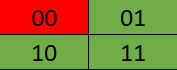
\includegraphics[width=67mm, keepaspectratio]{figures/sirf_sil1.png}\hspace{1cm}
	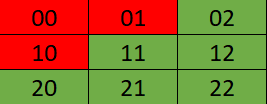
\includegraphics[width=67mm, keepaspectratio]{figures/sirf_sil2.png}\\\vspace{1cm}
	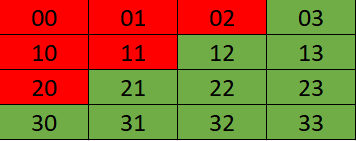
\includegraphics[width=67mm, keepaspectratio]{figures/sirf_sil3.png}\hspace{1cm}
	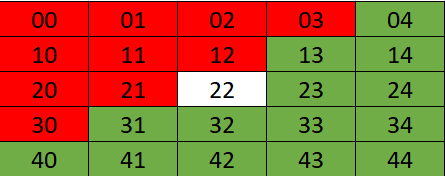
\includegraphics[width=67mm, keepaspectratio]{figures/sirf_sil4.png}
	\caption{Megengedett kombinációk az integritás szinteknek megfelelően, sorrendben SIL1, SIL2, SIL3, SIL4 \emph{Forrás}: SIRF 400}
	\label{fig:sirfSIL}
\end{figure}
\section{Top-down módszerek}
\subsection{Funkcionális analízis}
A funkcionális analízis (FA) egy alapvető módszer a rendszer kritikus funkciói megértéséhez és tervezéséhez.
Az FA elvégzése nélkülözhetetlen a RAMS menedzsmentben és a rendszertervezésben.
A vizsgálat célja, hogy információt adjon arról, ami befolyásolja a rendszer funkcióit és alapot nyújtson a RAMS menedzsmenthez.

Az FA még a specifikáció, modellezés, szimuláció, validáció és verifikáció lépéseinél is alkalmazható.
Ezért a funkcionális analízis gyakran fontos módszerként alkalmazzák a rendszer funkcionális struktúrájának meghatározására.
A funkcionális analízist általában az alábbi két megközelítésben alkalmazzák:
\begin{itemize}
    \item Struktúrált Analízis és Design módszer (SADT\footnote{Structured Analysis and Design Technique})
    \item Funkcionális Analízis Rendszer módszer (FAST\footnote{Functional Analysis System Technique})
\end{itemize}
SADT-ot több iparágban is alkalmazzák. 
Ez egy diagramszerű koncepció, mely segítségével megérthető és leírhatók a rendszer funkcionális viselkedési és interfészei.
A módszer számos elemet szolgáltat az aktivitások és adatfolyamok reprezentálására és nyilakat ezek kapcsolataihoz, ahhogy az alábbi \ref{fig:sadt} ábrán látható, ami egy példa az SADT-ra.

\begin{figure}
    \footnotesize
    \centering
    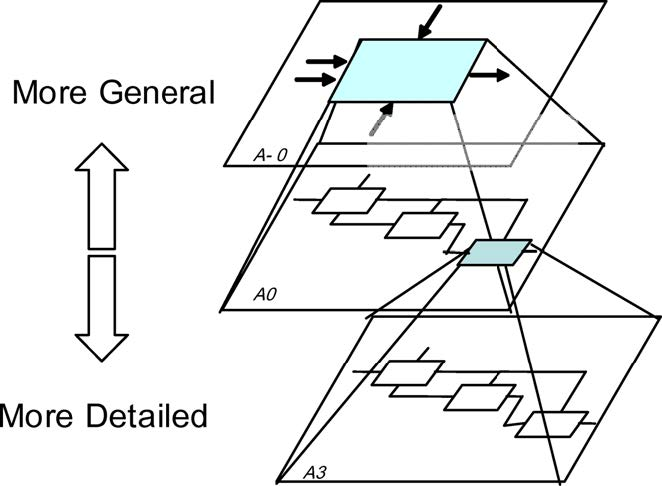
\includegraphics[width=100mm, keepaspectratio]{figures/roh2007.jpg}
    \caption{SADT modell (Forrás: Roh, 2007\cite{doi:10.1080/13675560701478240})}
    \label{fig:sadt}
\end{figure}

A FAST Charles Bytheway fejlesztette ki 1964-ben. Ezt a módszert is sok iparág használja.
A FAST-ot azokban a szituációkban lehetséges felhasználni, ahol a funkciókat logikai sorozatban lehet ábrázoloni, ezáltal priorizálni őket és megvizsgálni a függőségeit.
Ez a módszer nem alkalmas funkcionális problémák megoldására, inkább feltárni a rendszer alapvető funkcionális karakterisztikáit.
Az \ref{fig:fast} ábra egy példa a FAST modellre Kaufmann (1982) által.

\begin{figure}
    \footnotesize
    \centering
    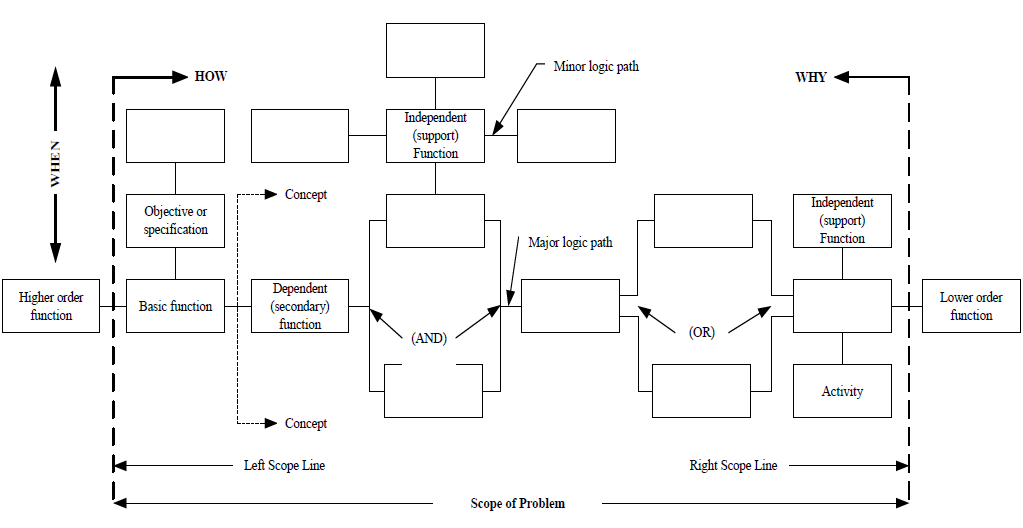
\includegraphics[width=150mm, keepaspectratio]{figures/fast.png}
    \caption{FAST modell (Forrás: Kaufmann, 1982, \cite{Kaufmann:1982})}
    \label{fig:fast}
\end{figure}

\subsection{Hibafa analízis}
A Hibafa analízis (FTA\footnote{Fault Tree Analysis}) egy szisztematikus, deduktív és logaikai módszer a rendszerhiba (Top event) okainak feltárására, modellezésére, vizsgálatára.
Az FTA-t lehet az egyek legmegbízhatóbb eszköznek tekinteni a hiba eset logaikai kiértékelésében biztonsági és megbízhatósági szempontból. \cite{Ericson}

A hibafát H. Watson és Allison B. Mearns fejlesztette ki 1962-ben, akik együtt dolgoztak a US Bell Company laboratóriumában. Később a Boeing Company is elkezdte használni a módszert, hogy meghatározza a biztonsági faktorokat, melyek fegyverrendszerekre lehetnek hatással.
Az 1960-as években a kereskedelmi repülés, '70-es években a nukleáris energiaipar, '80-as években a vegyipar, '90-es években közlekedési ipar is elkezdte használni a módszert biztonságosság és megbízhatóság felmérésére (Ericson, 1999).

Az analízis az előfordulható hibamódok egy részhalmazára fokuszál, különös tekintettel azokra, amik katasztrofális hibát okozhatnak.
A kapuk (gate), események (event) és vágások (cut set) jelentik a legfőbb elemzési pontjait.
A logikai diagramm - 'ÉS' és 'VAGY' kapuk - adja meg a FTA eredményét.
A hibaesetek adják meg a kapuk bemeneteit és a vágások adják meg azoknak a hibaeseteknek halmazát, ami rendszerhibát okozhat.
Az FTA-t szokás az FMECA\footnote{Failure Mode Effect and Criticallity Analysis}-val, Markov analízissel és ETA\footnote{Event Tree analysis}-val együttesen használni, hogy elfedjék az FTA limitációit (Stapelberg, 2008; BE EN 60812, 2006).

\begin{figure}
    \footnotesize
    \centering
    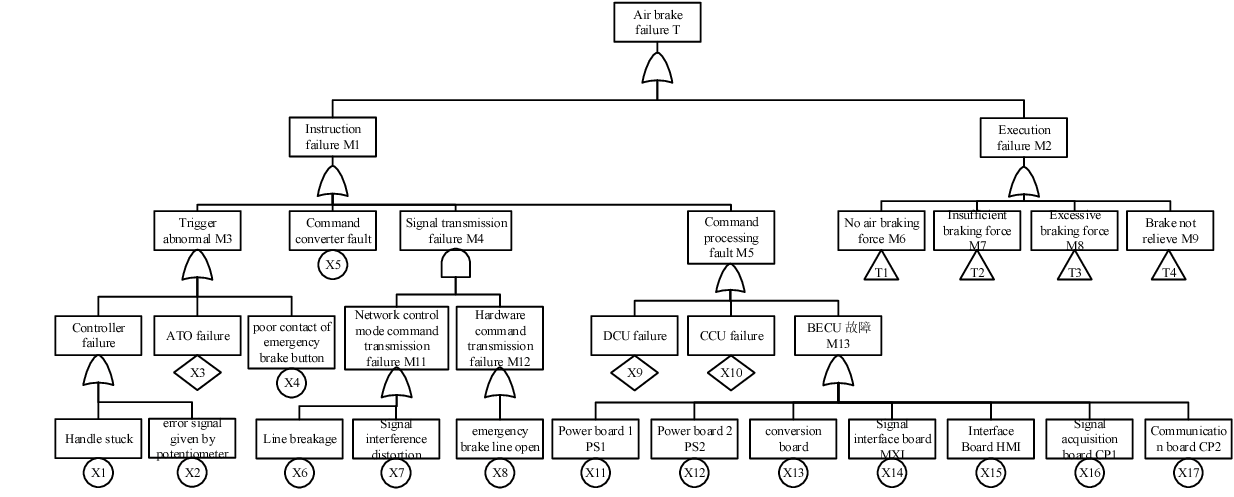
\includegraphics[width=150mm, keepaspectratio]{figures/fta1.png}
    \caption{Egy hibafa példa pneumatikus fékrendszer meghibásodásához (Forrás: Long, 2017 \cite{Long2017BrakingSM})}
\end{figure}

\subsection{Megbízhatósági blokkdiagram analízis}
A Megbízhatósági blokkdiagram (RBD\footnote{Reliability Block Diagram}) egy vizuális elemzési módszer aminek segítségével könnyen reprezentálható a rendszer logikailag összekötött struktúrája.
Az RBD blokkjai ábrázolják a rendszer eredményes működését. Az elemzés különböző szinten jelentkezhet, mind kvalitatív, mind kvantitatív formában (BS EN 61078, 2006; BS EN 60300-3-1, 2004).

A diagramm felépíthető egyenesen a rendszer funkciónális modelljéből, ami szisztematikusan megjeleníti a funkcionális utakat.
Sok különböző rendszerkonfigurációt képes kifejezni, például, soros, párhuzamos, rendundáns, ,,standby'' stb., ahogy az az \ref{fig:rdb} ábrán is látszik.
Az RBD-t általában abban az esetben használják, amikor különböző változatait és komprumisszumait kell értékelni megbízhatósági és elérhetőségi szempontból.
\begin{figure}
    \footnotesize
    \centering
    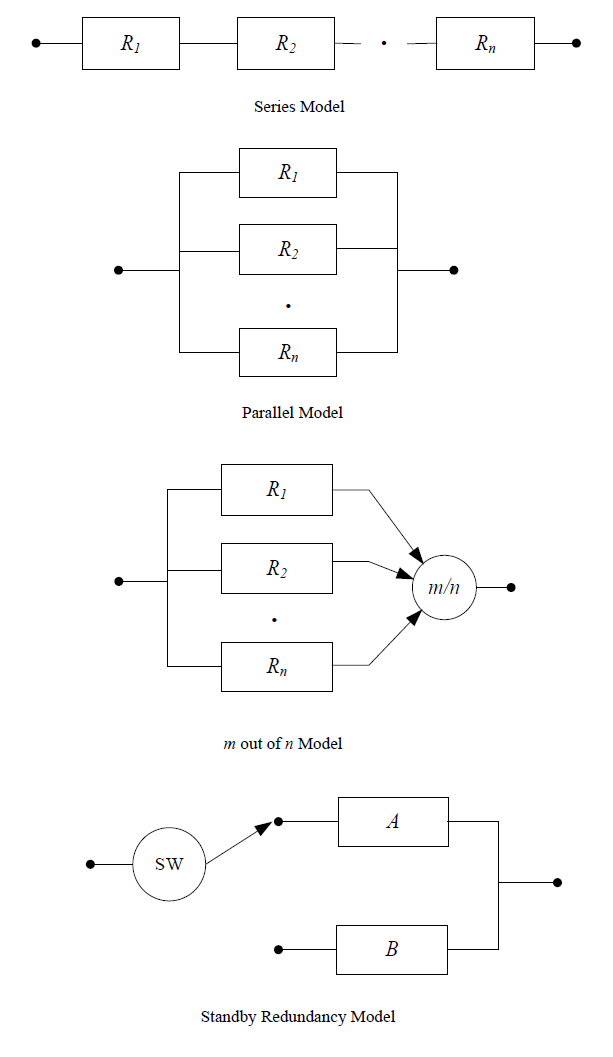
\includegraphics[width=80mm, keepaspectratio]{figures/rbd1.png}
    \caption{Különböző RDB modellek (Forrás: BS EN 61078, 2006)}
    \label{fig:rdb}
\end{figure}

\subsection{Közös hibaforrás azonosítás}


\section{Bottom-up módszerek}
\subsection{FMEA analízis}
Az Hibamód és hatás analízis (FMEA\footnote{Failure Mode and Effect Analysis}) egy biztonságossági és megbízhatősági kiértékelő módszer, ami képes felmérni a rendszer összem komponensének összes potenciális hibamódját, ami kihathat az egész rendszer teljesítményére.
A módszer továbbá azonosítja azokat a módszereket is, amikkel elkerülhetők a hibamódok és hogyan lehetséges csökkenteni azok hatását.

A módszert eredetileg FMECA\footnote{Failure Mode Effect and Criticality Analysis} néven említették, amiben a ,C' betű a hibamód kritikusságát jellemezte.
Bár a két módszert gyakran szinonímaként használják, teljesen más a megközelítésük.
Általában az FMEA-t a hibamód hatásának súlyosságát minősíti, míg az FMECA a hibamód frekvenciáját is megvizsgálja a súlyosság mellett.
A súlyosság és a frekvencia kombinációját a rendszer kritikusságnak vagy kockázatának nevezik (MIL-STD-1629A, 1980).

A módszer során minimum a következő nyolc információt kell megállapítani:
\begin{enumerate}
    \item Hibamódok (Failure mode)
    \item A hibamód hatása a rendszerre
    \item A hibamód miatt bekövetkezett rendszerszintű hiba
    \item A veszélyek baleseti hatása
    \item A hibamód és/vagy veszély okozati tényezőit
    \item Hogyan lehet a hibamódot detektálni
    \item Javaslatok
    \item A felderített veszély kockázatát
\end{enumerate}

A módszert több szempontból is el lehet végezni.
Ez lehetnek Funkcionális megközelítés, Struktúrális megközelítés és a ,,hibrid'' megoldás.
Az első megközelítésben a funkciók céljának lehetséges hibás működését veszi figyelembe.
Ez a módszer alkalmazható szoftverek esetében is.

A második megközelítés leginkább hardver elemeken végzett lehetséges hibamódokra öszpontosít.
A ,,hibrid'' megközelítés először a funkcionális analízissel kezdődik, aminek fókusza átvált a hardverre (Ericson, 2005).

Lehetséges példák a funkcionális hibamódokra:
\begin{itemize}
    \item A funkció nem működik
    \item A funkció nem megfelelően működik
    \item A funkció idő előtt hajtódik végre
    \item A funkció hibás vagy félrevezető információt szolgáltat
    \item A funkció nem hibásodik meg biztonságosan
\end{itemize}
Lehetséges hardver hibamód kategóriák:
\begin{itemize}
    \item Teljes meghibásodás
    \item Részleges meghibásodás (például: tolerancián kívül)
    \item Időszakos meghibásodás
\end{itemize}
Lehetséges hardver hibamódok:
\begin{itemize}
    \item Szakadás
    \item Rövidzárlat
    \item Tolerancián kívül
    \item Szivárgás
    \item Meleg felület
    \item Elhajlás
    \item Túl/alulméretezett
    \item Megrepedt
    \item Rideg
    \item Elmozdult
    \item Korrodált
    \item stb.
\end{itemize}
Lehetséges hibamódok szoftvereknél:
\begin{itemize}
    \item A szoftver funkció meghibásodik
    \item A funkció hibás eredményt szolgáltat
    \item A funkció idő előtt meghívódik
    \item Elküldetlen üzenetek
    \item Túl korán/későn küldött üzenet
    \item Hibás üzenet
    \item Megáll vagy összeomlik a szoftver
    \item Belső kapacitásoknál többet igényel a szoftver
    \item Szoftver ,,startup'' hiba
    \item Lassú válaszidő
\end{itemize}

\subsection{HAZOP analízis}
A Hazard and operability study (HAZOP) analízis egy szisztematikus vizsgálat, ami feltárja és tanulmányozza egy rendszer potenciális veszélyeit és üzemeltetési problémáit.
Rendezett, struktúrált és módszeres folyamatot követ\cite{Ericson}.

A HAZOP-ot az angol Chemical Industry Insitute formalizálta a '70-es években.
A módszer széleskörben elterjedt számos biztonságkritikus iparágban, mint a vegyipar.

A módszertan néhány útmutató szó segítségével próbálja rávezetni a vizsgálót a problémás részekre.
Ilyen útmutató szavak lehetnek például: 'Nem', 'Több', 'Kevesebb', 'Fordítva' stb., mint az látható a \ref{tab:hazop}. táblázatban.
A HAZOP módszer leghatékonyabb a részletes terv kidolgozása után, mert ilyenkor már működtetési problémákat is feltár.
A \ref{tab:hazop} táblázat egy vonat ajtó működési problémáit tárja fel egy peronnál HAZOP segítségével.

\begin{table}[!ht]
    \footnotesize
    \begin{tabular}{|l p{25mm} p{25mm} p{25mm}|}
        \toprule
        Útmutató & Eltérés & Ok & Okozat \\
        \midrule
        Nem & Az ajtó nem nyílik & Hibás mechanizmus & Nem tudnak leszállni az utasok \\
        \midrule
        Több & Az ajtó túl korán nyílik & Kezelő hibázik & Lehetséges sérülés \\ 
        \midrule
        Kesevebb & Csak egy ajtó nyílik ki & Hibás mechanizmus & Korlátozott leszállás, lehetséges sérülés\\ 
        \midrule
        Ugyan úgy & A vonat mindkét oldalán nyílik az ajtó & Hiba a vezérlőben & Lehetséges sérülés, ha a rossz oldalon szállnak le\\ 
        \midrule
        Más mint & Rossz oldalon nyílik az ajtó & Vezérlő hiba & Lehetséges sérülés, ha a rossz oldalon szállnak le \\
        \bottomrule
    \end{tabular}
    \caption{Egy példa a HAZOP használatára}
    \label{tab:hazop}
\end{table}

\subsection{LOPA}
Layer of Protection Analysis-t (LOPA) először az 1990-es évek végén kezdték el alkalmazni a vegyiparban.
Ahogy a módszert egyre szélesebb körben alkalmazták, az AIChE Center of Chemical Process Safety (CCPS) elkezdett irányelveket kiadni hozzá.
Később más szervezetek is elkeztek a LOPA-ra hivatkozni, mintpéldául az IEC\footnote{International Electrotechnical Commission} vagy az ISA\footnote{International Society of Automation} \cite{WILLEY201412}.

A layer of protection analysis megfeleltethető az Event Tree Analysis (ETA) egy megfelelő adaptációjának\cite{HRRS}, lásd: \ref{fig:lop_eta}. ábra.

\begin{figure}
    \footnotesize
    \centering
    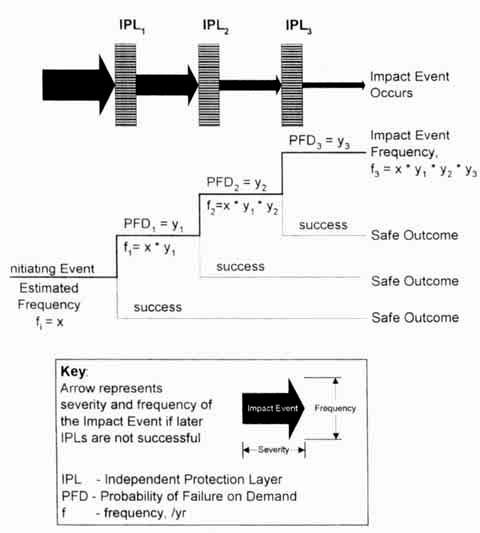
\includegraphics[width=100mm, keepaspectratio]{figures/lopa.jpg}
    \caption{LOPA analízis esemény fával ábrázolva (Forrás: \cite{LOPA1})}
    \label{fig:lop_eta}
\end{figure}

A LOPA analízist általában közvetlenül a HAZOP tanulmány után készítik el, de még a hibafa analízis előtt.

\subsubsection{LOPA koncepciója}
A LOPA koncepciója összefoglalva:
\begin{enumerate}
    \item Megtalálni azokat az eseményeket, amelynek a külvilágra hatása van. Meghatározni ezek hatását(emberek, környezet, tulajdon)
    \item Felsorolni a ezeknek az eseményeknek a kezdeti okát.
    \item Megbecsülni a kezdeti okok frekvenciáját.
    \item Minden ok-okozati párra felsorolni a független védelmi rétegjét (IPL\footnote{Independent Protection Layer}).
    \item Meghatározni a hiba valószínűségét minden IPL-nek.
    \item Kiszámolni a mérsékelt előfordulási frekvenciát az összes ok-okozati párra.
    \item Összevetni a kapott frekvenciát az előre definiált tűrhető veszéllyel.
\end{enumerate}

Ha mindezek után a kapott érték nem teljesíti a kritériumot az alábbi opciókat lehet végrehajtani:
\begin{itemize}
    \item További rétegeket adunk a rendszerhez.
    \item Növeljük valamelyik réteg SIL szintjét (azaz csökkentjük annak frekvenciáját)
    \item Újratervezzük a folyamatot vagy
    \item még részletesebb vizsgálatot folyatatunk, pédául: Hibafa Analízissel.
\end{itemize}
%----------------------------------------------------------------------------
\chapter{\caseStudy} \label{chap:cs}
%----------------------------------------------------------------------------

\section{A tanulmány háttere}
Az esettanulmány során egy kitalált, de mégis valósághű vasúti fékrendszert tervezek és elemzem biztonsági szempontból.

A vasútipart és ezzel együtt a vasútifék-technológiát az utóbbi időben rohamos fejlődés határozta meg. 
Számos működési elv elérhető az iparágban (pneumatikus, hidraulikus, elektro-pneumatikus, elektro-hidraulikus, elektromágneses), amelyeknek mind meg van a maga előnye és hátránya.

Ebben a dolgozatban egy összetett integrált fékrendszer megoldást szeretnék modellezni, mely rendelkezik egy fékvezérlő berendezéssel.
Ezért az elavultnak számító és mára leginkább csak a vasúti teherszállításban - az egyszerűsége és költséghatékonysága miatt - használt pneumatikus és a szintén tisztán fizikai elven működő hidraulikus rendszereket nem találtam alkalmasnak a dolgozat témájához.

Napjainkban fontos téma, többek között a globális felmelegedés és a ${CO}_2$ kibocsátás visszaszorítása - melyek részletei és elemzése nem képezik ennek a dolgozatnak részét - miatt, a tömegközlekedés.
A vasútipar emberek szállítmányozására alkamas része is több alrészre bontható, nagysebességű(>300 km/h)/intercity vonatok, 
regionális/ingázó vonatok (pl: Budapesti HÉV), metró, könnyű vasúti vonatok/villamosok.

A dolgozat során egy modern alacsonypadlós városi tömegközlekedésre alkalmas villamos rendszerén keresztül szeretném bemutatni a modell alapú rendszertervezés (Model-based Systems Design, MBSD) módszertanait és az elkészült rendszer biztonsági és megbízhatósági analízisét. 
Mivel az alacsonypadlós villamosokon véges hely áll rendelkezésre, ezért egy kompakt megoldásra van szükség. 
Továbbá, biztosítani kell bármely közlekedési helyzetben a szerelvény biztonságos és optimális lassulását, megállását.

\section{Vasúti jármű fékrendszer} \label{sec:vjfr}
A vasúti járművek fékei rendkívül összetett folyamatot alkotnak és specifikusak a vasúti járművekre.
A fékrendszer egy fontos biztonsági funkció, mely szabályozza a jármű sebességét és megállítja egy fix helyen, mint például egy állomásnál \cite{13452-1}.

Egy vasúti fékrendszernek a következő célokat kell teljesíteni:
\begin{itemize}
    \item Lassítani vagy megállítani a mozgó vonatot
    \item Biztosítani az álló járművet
    \item Kontrollálni a jármű sebességét lejtőn
\end{itemize}

Ezekhez számos funkciót kell teljesítsen a rendszer, melyek a kövezkezők:
\begin{itemize}
    \item üzemi fék
    \item vészfék
    \item biztonsági fék
    \item biztosító fék
    \item parkoló fék
    \item opcionálisan kerékcsúszás prevenciós rendszer (WSP\footnotemark{})
\end{itemize}

\subsection{Üzemi fék}
Az üzemi fék az elsődleges fékrendszer normál üzemi állapotban.
Ezt a rendszert általában a jármű vezetője és/vagy a járművet vezető autómatika kezeli, hogy az általuk kívánt sebességre szabályozzák a vasúti szerelvényt.

\subsection{Vészfék}
Ezen funkció legfőbb célja az utasok, személyzet és a vasutat nem használók biztonságának maximalizálása.
Továbbá ez a funkció képes a lehető leghamarabb nyugalmi állapotba hozni a szerelvényt.

\subsection{Biztonsági fék}
Európában és a világ számos pontján kötelező olyan berendezéssel ellátni az új járműveket, amely a szerelvény esetleges menetközben több részre szakadásakor
a jármű összes részét biztonságosan megállásra kényszeríti. Ezt a funkciót nevezik biztonsági fékmechanizmusnak.

\subsection{Biztosító fék}
Ez a funkció felel a jármű egyhelyben tartásáért, amikor megáll a jármű egy állomáson.

\subsection{Parkoló fék}
A parkoló fék felel a jármű helyben tartásáért, miközben a jármű üzemen kívül van. 

\subsection{Kerékcsúszás prevenciós rendszer}
A WPS\footnotemark[\value{footnote}] egy olyan rendszer, amely optimalizálja a fékteljesítményt és védelmet nyújt a kerék és a sín sérülése ellen gyenge súrlódási viszonyok között.
\footnotetext{Wheelslide Protection System}




%----------------------------------------------------------------------------
\chapter{\modeling}
%----------------------------------------------------------------------------
\section{Architektúra}

\begin{figure}
    \centering
    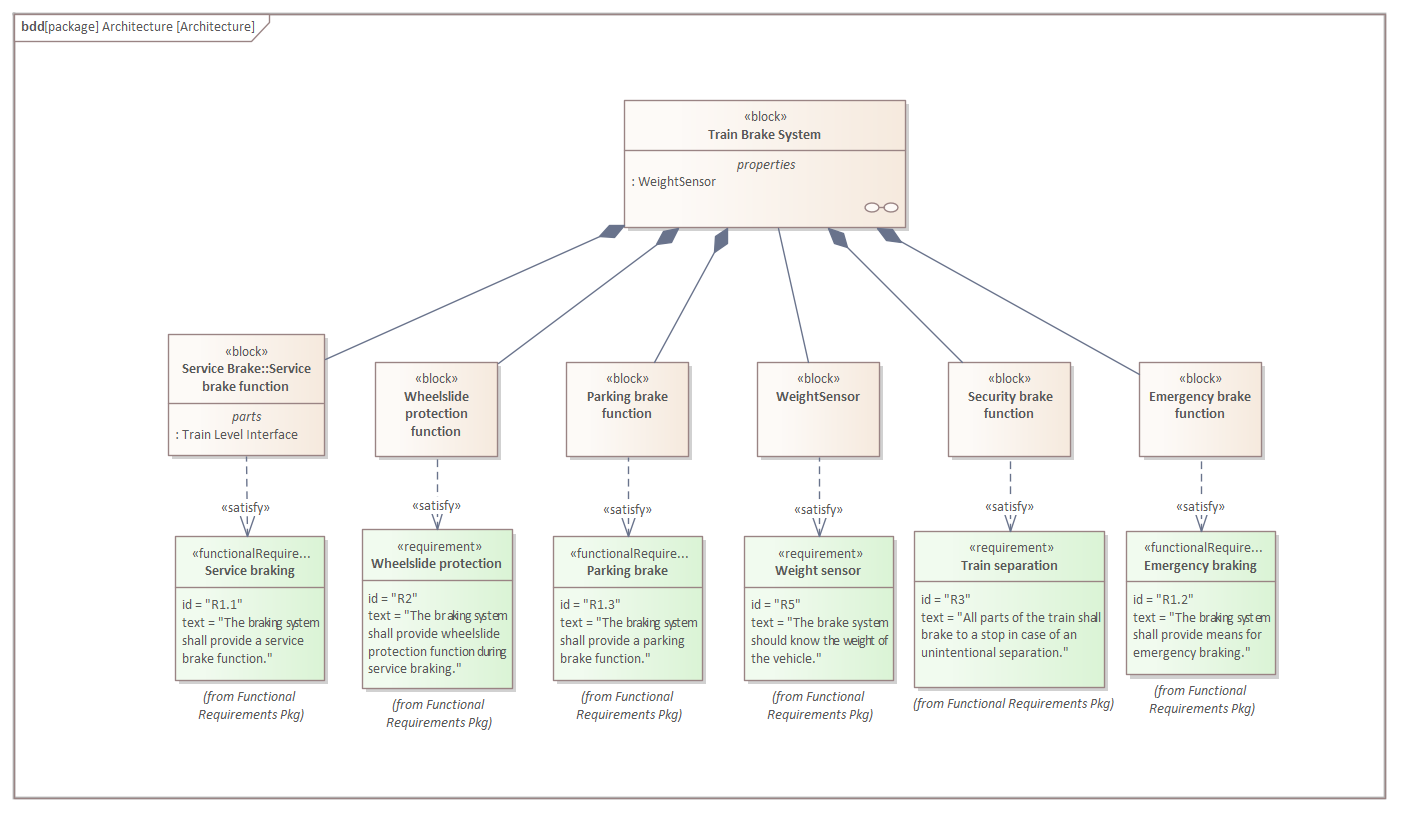
\includegraphics[width=150mm, keepaspectratio]{figures/Architecture.png}
    \caption{A fékrendszer fő architektúrája, a magas-szintű követelményekkel hozzárendelve.}
    \label{fig:architecture}
\end{figure}
%----------------------------------------
\chapter{\analysis}\label{chap:analysis}
%----------------------------------------
A dolgozat során elkészített rendszer terv csak akadémiai célokat szolgál, ezért nem követi teljes mértékben a valóságot.
Teljes mértékben kielégítő biztonsági vizsgálatot ezért nem lehet végezni a rendszeren.
A következő részekben inkább szeretném bemutatni egyes elemzési módszerek lényegét, alkalmazhatóságát mintsem egy valós projekt szerinti precíz megvalósítsát.

Mivel a biztonságosság kiemelten fontos témakör az iparágban, ezért az elemzésben a valósághoz hasonló értékek szerepelnek, de ezen értékek kitaláltak és reprezentatív jellegűek.
Az analízis során feltárt kockázatok besorolását az EN 50126\cite{EN50126-1} első részében leírt kockázat mátrix kalibrációs táblázatai szerint határoztam meg.

A frekvenciák besorolásához a \ref{tab:freqency}. táblázatot készítettem el.
Ennek segítségével besorolhatók egyes kvantitatív értékek az elfogadási mátrixban.

Továbbá a \ref{tab:serverity} és a \ref{tab:risk} segédtáblázatok alapján már meghatározható az a táblázat, amely a balesetek súlyossága és a hiba előfordulásának gyakorisága alapján meghatározza a kockázat elfogadásának lehetőséget.
Ezt a táblázatot reprezentálja a \ref{tab:risk_mat} táblázat.

Az elemzések további szakaszaiban ezen táblázatok felhasználása szerint lesznek meghatározva az előforduló hibák.
\begin{table}
    \footnotesize
    \centering
    \begin{tabular}{ |c|p{10em}|p{8em}|p{10em}| }
        \hline
        Frekvencia szint & Leírás & Frekvencia példa egy 24 órában működő eszköznél & Frekvencia \\
        \hline
        Gyakori & Az esemény gyakran bekövetkezik & Több mint egyszer 6 hónapos időszak alatt & $f \leq 1\times10^{-3}$ \\
        \hline
        Valószínű & Az esemény várhatóan többször bekövetkezik & Hozzávetólegesen egyszer 6 hét és egy év között & $ 1\times10^{-3} < f \leq 1\times10^{-4} $ \\
        \hline
        Alkalmi&Az esemény több alkalommal bekövetkezhet & Hozzávetőlegesen egyszer egy év és 10 év között & $1\times10^{-4} < f \leq 1\times10^{-5}$ \\
        \hline
        Ritka&Valószínű, hogy bekövetkezik valamikor a rendszer élettartama során & Hozzávetőlegesen egyszer 10 év és 1 000 év között & $1\times10^{-5} < f \leq 1\times10^{-7}$ \\
        \hline
        Valószínűtlen&Velószínűtlen a bekövetkezés, de megtörténhet & Hozzávetőlegesen egyszer 1 000 év és 100 000 év között & $1\times10^{-7} < f \leq 1\times10^{-9}$ \\
        \hline
        Erősen valószínűtlen&Az esemény vélhetően egyszer sem fog bekövetkezni & Hozzávetőlegesen egyszer 100 000 éveben vagy kevesebbszer & $1\times10^{-9} < f$ \\
        \hline
    \end{tabular}
    \caption{A veszély besorolási mátrix frekvencia tartomány kalibrációja. Saját adatok, a \cite{EN50126-1} alapján.}
    \label{tab:freqency}
\end{table}

\begin{table}
    \footnotesize
    \centering
    \begin{tabular}{ |c|p{10em}|p{10em}| }
        \hline
        Súlyossági kategória & Következmények az emberekre / környezetre                                                                                                     & Következmények a szolgáltatásokra \\ \hline
        Katasztrofális       & Emberek tömegét befolyásolja és többek halálához vezethez és/vagy  súlyos környezeti károsodás      & -                                 \\ \hline
        Kritikus             & Emberek kis számát befolyásolja és legalább egy halálesetet okoz és/vagy  nagy környezeti károsodás & Egy fontos rendszer elvesztése    \\ \hline
        Marginális           & Nincs lehetőség halálesetre, cask súlyos vagy könnyű sérülések és/vagy kis környezeti károsodás     & Súlyos rendszer sérülés           \\ \hline
        Jelentéktelen        & Lehetséges könnyű sérülés                                                                                                                     & Jelentéktelen rendszer sérülés    \\ \hline
    \end{tabular}
    \caption{Súlyossági kategóriák, az EN 50126-1 alapján.}
    \label{tab:serverity}
\end{table}

\begin{table}
    \footnotesize
    \centering
    \begin{tabular}{ |c|p{20em}| }
        \hline
        Kockázat elfogadási kategória & Végrehajtandó intézkedések\\ \hline
        Tolerálhatatlan & A kockázatot meg kell szüntetni \\ \hline
        Nem kívánatos & A kockázatot csak abban az esetben lehet elfogadni, ha annak csökkentése nem lehetséges \\ \hline
        Tolerálható & A kockázat tolerálható és elfogadható megfelelő ellenőrzéssel (például: karbantartási útmutatók vagy szabályok) \\ \hline
        Elhanyagolható & A kockázat minden további nélkül elfogadható \\ \hline
    \end{tabular}
    \caption{Kockázat elfogadási kategóriák, az EN 50126-1 alapján.}
    \label{tab:risk}
\end{table}

\begin{table}
    \centering
    \begin{tabular}{|l|l|l|l|l|} 
        \hline
        Előfordulási frekvencia & \multicolumn{4}{l|}{Kockázat elfogadási kategória}                    \\ 
        \hline
        Gyakori                 & Nem kívánatos  & Tolerálhatatlan & Tolerálhatatlan & Tolerálhatatlan  \\ 
        \hline
        Valószínű               & Tolerálható    & Nem kívánatos   & Tolerálhatatlan & Tolerálhatatlan  \\ 
        \hline
        Alkalmi                 & Tolerálható    & Nem kívánatos   & Nem kívánatos   & Tolerálhatatlan  \\ 
        \hline
        Ritka                   & Elhanyagolható & Tolerálható     & Nem kívánatos   & Nem kívánatos    \\ 
        \hline
        Valószínűtlenű          & Elhanyagolható & Elhanyagolható  & Tolerálható     & Nem kívánatos    \\ 
        \hline
        Erősen valószínűtlen    & Elhanyagolható & Elhanyagolható  & Elhanyagolható  & Tolerálható      \\ 
        \hline
        \multicolumn{1}{l|}{}   & Jelentéktelen  & Merginális      & Kritikus        & Katasztrofális   \\ 
        \cline{2-5}
        \multicolumn{1}{l|}{}   & \multicolumn{4}{l|}{A baleset súlyossága}                             \\
        \cline{2-5}
        \end{tabular}
    \caption{Kockázat elfogadási mátrix.}
    \label{tab:risk_mat}
\end{table}

\section{HAZOP analízis}
A vizsgálatot HAZOP tanulmány készítésével kezdtem.
Ez alkalmas a rendszer platform modellje alapján előre meghatározott módszertan szerint szisztematikusan eltárni az adott alrendszerek tervezettől való eltérő viselkedéseinek feltárására.

A vizsgálat segéd szavak segítségével vezeti rá az elemző (csapat) gondolkodását a lehetséges eltérésekre.
A módszertan által nyújtott lehetséges szavak csak egy részét felhasználva, a következő iránymutató szavak lettek felhasználva a dolgozatban: (1) NEM (NO), (2) KEVESEBB (LESS), (3) TÖBB (MORE).

Ezután két alrendszert vizsgáltam a módszertan szerint, ezek pedig a hidraulikus fékolló (Hydraulic Caliper) és a vezérlő elektronika (Control Electronics).

A HAZOP tanulmány eredményessége nagyban függ az azt végrehajtó csapat kreativitásán, ezért nem feltételezhető az adott egység minden egyes hibaforrásának észlelése/feltárása.

Az általam elvégzett vizsgálat során a \ref{tab:hazop_vizsg}. táblázatban látható potenciális eltérésekre jutottam.


\begin{table}
    \centering
    \begin{tabular}{ |p{18mm}|p{15mm}|p{20mm}|p{20mm}|p{25mm}|p{25mm}| }
        \hline
        Item & Guide word & Deviation & Cause & Consequence & Existing controls \\
        \hline
        Hydraulic Caliper & NO & No brake force & Caliper failure & Longer braking distance / possible crash with traffic & Recommended service interval / routine checks \\
        & LESS & Reduced brake force & Worn out brakepads & Longer braking distance / possible crash with traffic & Recommended service interval / routine checks \\
        & LESS & Reduced brake force & Control loop failure & Longer braking distance / possible injury to multiple people & - \\
        & MORE & More brake force & Failure of pressure generation & Possibility of train stuck on track / minor injuries & - \\
        \hline
        Control Electronics & NO & No input voltage & Train battery line failure & Train stuck on track & - \\
        & MORE & Higher input voltage than specified & Train battery line failure & Control electronics power supply failure & Over voltage protection \\
        & MORE & Higher brake demand than requested & Control output stuck at low & Possibility of train stuck on track / minor injuries & Under voltage protection \\
        & LESS & Lower input voltage than specified & Train battery line failure & Possibility of train stuck on track / minor injuries & - \\
        & LESS & Lower brake demand than requested & Control output stuck at high & Longer braking distance / possible injury to multiple people & Error signaling \\
        & LESS & Lower brake demand than requested & Wheelslide protection lowers the brake demand for a long time & Longer braking distance / possible injury to multiple people & WSP watchdog \\
        \hline
    \end{tabular}
    \caption{HAZOP vizsgálat a hidraulikus fékolló és vezérlő elektronika komponensekre.}
    \label{tab:hazop_vizsg}
\end{table}

\section{LOPA analízis}

\section{FTA}
\chapter{Összefoglalás}
A szakdolgozat során felkutattam számtalan a biztonsági analízishez használt módszert.
Ezen módszerek nagyrésze már szerepel a vasútipari szabványok valamelyikében, de más iparából is származott hasznos technológia.

A módszerek között megkülönböztettem lehetséges Top-down és Bottom-up irányú eszközöket is, leírva azok előnyét a fejlesztés lépéseinek támogarása során.

A dolgozat során bemutattam a modell-alapú rendszerfejlesztés pár lehetőségét a vasútiparra tekintve.
Elkészült a fékrendszer funkcionális modellje/architektúrája.
A fejlesztés során bemutattam a funkcionális dekompozíció lépéseit és ezáltal eljutottam egy kinevezett funkció (üzemi fék) alacsonyabb szintjeihez.

A funkcionális dekompozíció Top-down metodikája mellett elkészült a fékrendszer egy platform modellje.
Ebben bemutattam a Bottom-up módszertan felépítését, majd a kis komponensekből bemutattam a felépített rendszer modelljét.
Ezen a platform architektúrán már megjelentek a fizikai építőelemek és azok összeköttetéseik.

A modellezés végeztével az általam választott módszerekkel biztonsági analízist hajtottam végre az elkészült terveken.

Ebbeb bemutattam a HAZOP, a LOPA és az FTA módszereket.
A HAZOP egy magasszintű szisztematikus problémafeltáró eljárás, amely iránymutató szavak segítségével vezetett rá a lehetséges hibákra.
A LOPA átmenet a HAZOP és az FTA között. Segítségével egy egyszerű hibát rangsoroltam.
Az FTA összetett hibák elemzésére alkalmas eszköz aminek segítségével egy komplex alegység biztonsági vizsgálatát végeztem el.

\section{Javaslatok további munkára}
A jövőben szeretném részletesebben kidolgozni a rendszertervet.
Ebbe beletartozik a funkciók részletesebb dekompozíciója és ezen funkciók viselkedésének/kapcsolatainak modellezése.
Érdekes lehet még valós adatok/követelmények alapján készíteni a modelleket különböző tervezési kényszer mellett.

Továbbá szeretném tovább részletezni a biztonsági analízist is.
Ennél a feladatkörnél is érdekes lehet valós adatok/tények felkutatása és azok alapján végezni a vizsgálatot.
% Acknowledgements
%~~~~~~~~~~~~~~~~~~~~~~~~~~~~~~~~~~~~~~~~~~~~~~~~~~~~~~~~~~~~~~~~~~~~~~~~~~~~~~~~~~~~~~
%\include{content/acknowledgement}


% List of Figures, Tables
%~~~~~~~~~~~~~~~~~~~~~~~~~~~~~~~~~~~~~~~~~~~~~~~~~~~~~~~~~~~~~~~~~~~~~~~~~~~~~~~~~~~~~~
\listoffigures\addcontentsline{toc}{chapter}{\listfigurename}
\listoftables\addcontentsline{toc}{chapter}{\listtablename}

% Bibliography
%~~~~~~~~~~~~~~~~~~~~~~~~~~~~~~~~~~~~~~~~~~~~~~~~~~~~~~~~~~~~~~~~~~~~~~~~~~~~~~~~~~~~~~
\addcontentsline{toc}{chapter}{\bibname}
\bibliography{bib/mybib}


% Appendix
%~~~~~~~~~~~~~~~~~~~~~~~~~~~~~~~~~~~~~~~~~~~~~~~~~~~~~~~~~~~~~~~~~~~~~~~~~~~~~~~~~~~~~~
%\include{content/appendices}

%\label{page:last}
\end{document}
